% Teilaufgabe X

\section{Doppler-Verbreiterung und Linienbreite}
\label{sec:dopplerLine}

Bewegt sich ein angeregtes Atom mit der Geschwindigkeit $\vect{v}$, wird die Mittenfrequenz $\omega_0$ des vom Atom in Richtung des Wellenvektors $\vect{k}$ emittierten Lichtes für den ruhenden Beobachter aufgrund des Dopplereffekts verschoben [Abb. \ref{fig:dopplerLine}a]. Weiterhin fällt eine ebene Welle mit dem Wellenvektor $\vect{k}$ und der Frequenz $\omega$ auf ein Atom, welches sich mit der Geschwindigkeit $\vect{v}$ bewegt, erscheint die Frequenz $\omega$ im System des bewegten Atoms dopplerverschoben [Abb. \ref{fig:dopplerLine}b]. Damit ergibt sich für beide Fälle für die Emission (e) und Absorption (a) folgender Zusammenhang:
\begin{gather}
    \boxed{\omega_\mathrm{e,a} = \omega_0 + \vect{k}\cdot\vect{v}}~,
\end{gather}
das dadurch entstehende Dopplerprofil [Abb. \ref{fig:dopplerLine}c] ist dabei gaußverteilt (symmetrisch um $\omega_0$) mit der Dopplerbreite:
\begin{gather}
    \delta \omega_\mathrm{D} = \frac{2\omega_0v_\mathrm{w}}{c} \sqrt{\ln2}~,
    \label{eq:dopplerbreitevw}
\end{gather}
wobei $v_\mathrm{w}$ die wahrscheinlichste Geschwindigkeit im thermischen Gleichgewicht ist (aus Maxwellschen Geschwindigkeitsverteilung). Setzt man nun $v_\mathrm{w} = \sqrt{2k_\mathrm{B}T/m}$ in Gleichung \ref{eq:dopplerbreitevw} ein, erhält man:
\begin{gather}
    \boxed{\delta \omega_\mathrm{D} = \frac{\omega_0}{c}\sqrt{\frac{8k_\mathrm{B}T\ln2}{m}}}~.
    \label{eq:dopplerbreite}
\end{gather}
In Gleichung \ref{eq:dopplerbreite} lässt sich schnell erkenn, dass die Dopplerbreite $\delta \omega$ mit zunehmender Temperatur $T$ zunimmt und mit steigender Masse $m$ abnimmt. \cite{DemtroederAtome}
\begin{center}
    \captionsetup{type=figure}
    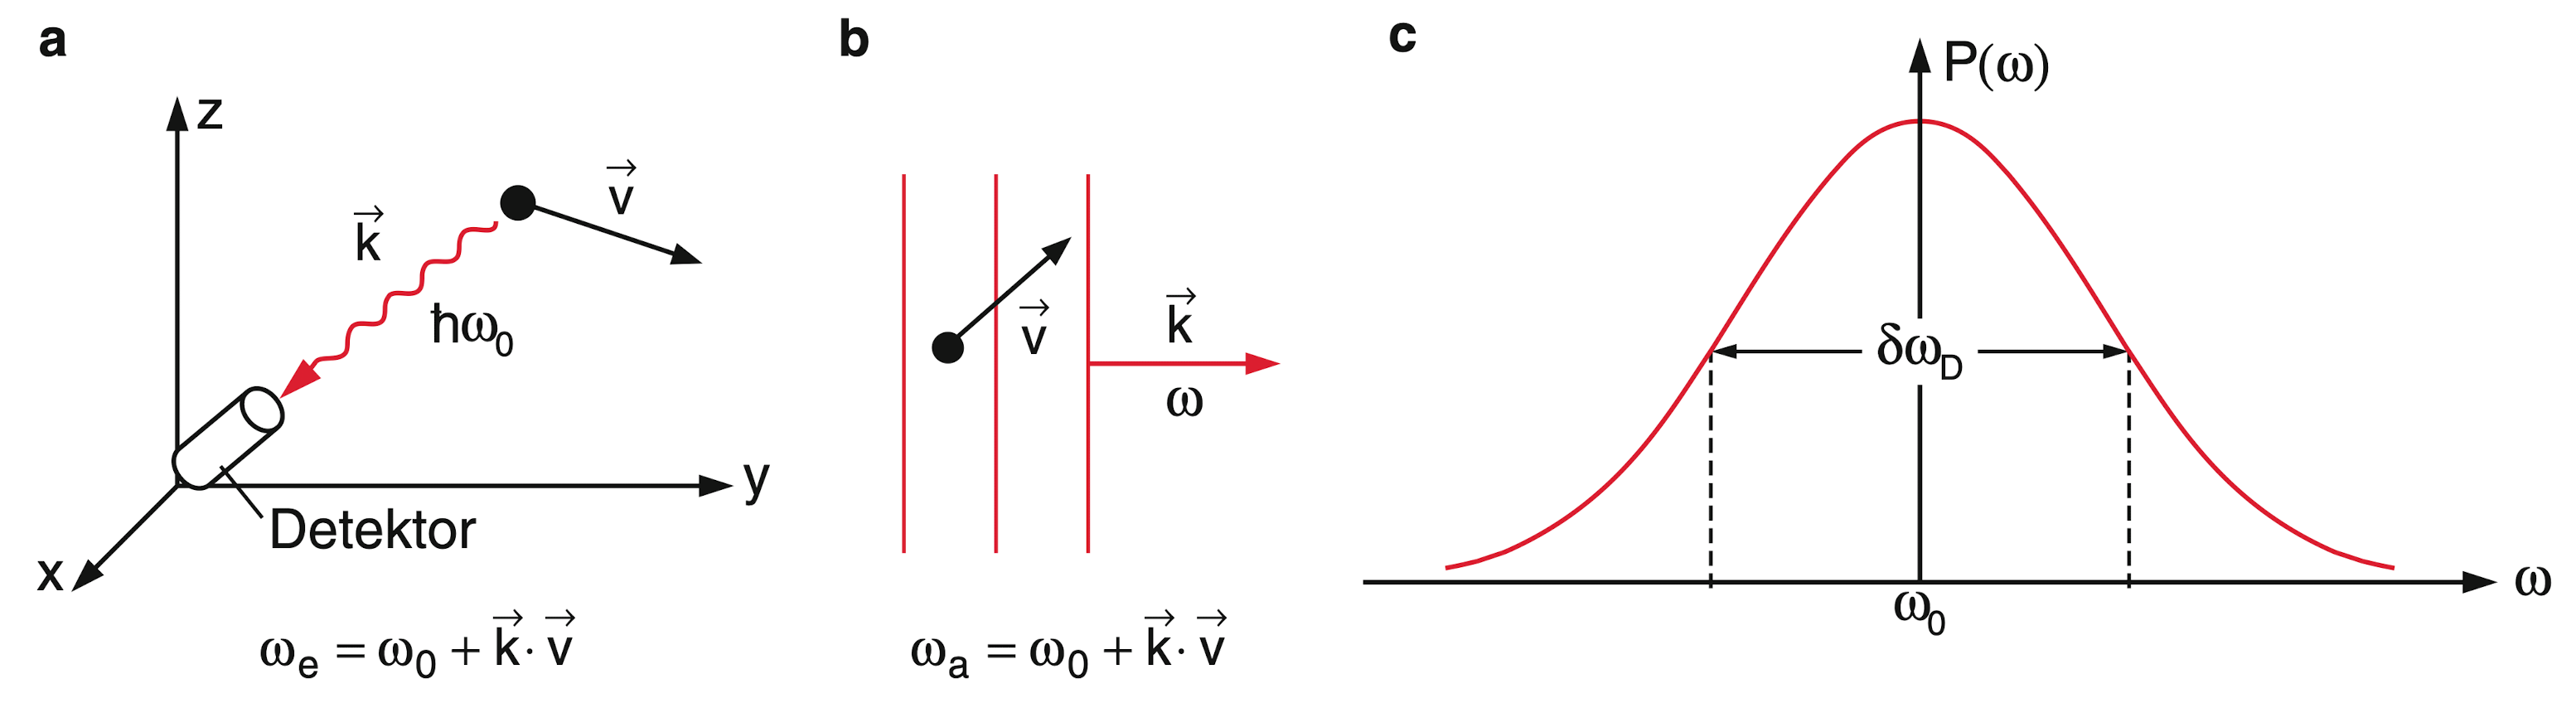
\includegraphics[width=\textwidth]{Bilder/Dopplerbreite.png}
    \captionof{figure}{Zum Dopplereffekt: \textbf{a} Verschiebung der Emissionsfrequenz $\omega_\mathrm{e}$, \textbf{b} Verschiebung der Absorptionsfrequenz $\omega_\mathrm{a}$, \textbf{c} Dopplerprofil einer Spektrallinie \cite{DemtroederAtome}}
    \label{fig:dopplerLine}
\end{center}
Des Weiteren kann ein die Dopplerbreite durch Stöße verbreitert werden, man spricht hierbei auch von Stoßverbreiterung. Dabei nähert sich zwei Atome mit unterschiedlichen Energieniveaus sich gegen seitig an und durch die Wechselwirkung wird so die Dopplerbreite vergrößert. \cite{DemtroederAtome}
\begin{itemize}
    \item \textbf{Homogene Linienbreite}:\\
    Homogene Linienbreite tritt auf, wenn die Wahrscheinlichkeit für die Emission bzw. Absorption von Licht mit Übergang $E_\mathrm{i} \rightarrow E_\mathrm{k}$ für alle Atome/Moleküle gleich groß ist. Die \textit{natürliche Linienbreite} ist ein Beispiel dafür. \cite{DemtroederLaser1}
    \item \textbf{Inhomogene Linienbreite}:\\
    Hängt die Wahrscheinlichkeit für die Emission bzw. Absorption des Lichts von der Geschwindigkeit des Atoms/Moleküls ab und damit für alle Atome/Moleküle \textbf{nicht} gleich groß. Die \textit{Doppler-Verbreiterung} ist eine solche inhomogene Linienbreite. \cite{DemtroederLaser1}
\end{itemize}